\RequirePackage[OT1]{fontenc} 
\documentclass[journal]{IEEEtran}

% *** CITATION PACKAGES ***
\usepackage[style=ieee]{biblatex} 
\bibliography{example_bib.bib}    %your file created using JabRef

% *** MATH PACKAGES ***
\usepackage{amsmath}

% Table Packages
\usepackage{booktabs}
\usepackage{tabularx}

% *** PDF, URL AND HYPERLINK PACKAGES ***
\usepackage{url}
% correct bad hyphenation here
\hyphenation{op-tical net-works semi-conduc-tor}
\usepackage{graphicx}  %needed to include png, eps figures
\graphicspath{{./images/}}
\usepackage{float}  % used to fix location of images i.e.\begin{figure}[H]

\begin{document}

% paper title
\newcommand{\LabNumber}{\#2}
\newcommand{\LabTitle}{Vector Impedance Measurements}

\title{RF Lab Module \LabNumber\ --- \LabTitle}
%\\ \small{Title of the session (you can be creative highlighting your findings)}}

% author names 
\author{Stephen Campbell
    % Student 2 First Name Last Name 
}% <-this % stops a space

% The report headers
\markboth{EE/CE 4202 Electrical and Computer Engineering Laboratory in Circuits. Lab \LabNumber, \today}%do not delete next lines
{Shell \MakeLowercase{\textit{et al.}}: Bare Demo of IEEEtran.cls for IEEE Journals}

% make the title area
\maketitle

% As a general rule, do not put math, special symbols or citations
% in the abstract or keywords.
\begin{abstract}
    In this lab, the Agilent E5071C Network Analyzer was used to measure S-parameters
    over broadband frequencies. The systematic calibration technique Short Open Load
    Thru was conducted at the beginning of the measurement process to mitigate the
    effects of systematic error.  Three major components had their S-parameters
    measured: a 50 Ohm Load, a 3dB attenuator, and a bandpass filter. These
    component tests allowed for familiarity with metrology in the RF environment to
    be gained.
\end{abstract}

\section{Introduction}

\IEEEPARstart{E}{xpertise}  in Short Open Load Thru (SOLT) calibration was
acquired through the preliminary portion of the RF Microwave Circuits
laboratory. This calibration utilizes 2 physical standards. One standard
contains the Short Open Load portions and the other contains the thru portion.
After calibration, the single port parameters of the 50 Ohm Load were assessed.
Next, the 2 port parameters of the 3 dB attenuator and bandpass filter were
measured.

\section{Analysis}

\textbf{How do vector impedance measurements (S-parameters) relate to magnitude
    and phase measurements at the input and output ports?}

A S parameters describes the power relationship between n ports. Specifically
for a 2 port network, a S parameter are equal to the ratio of the voltage seen
at the Output Port over the voltage seen to be coming out of the input port. S
parameters are complex because they take into account the phase difference
between the input and output voltage waves as well as the magnitude.

\begin{figure}[hbp]
    \centering
    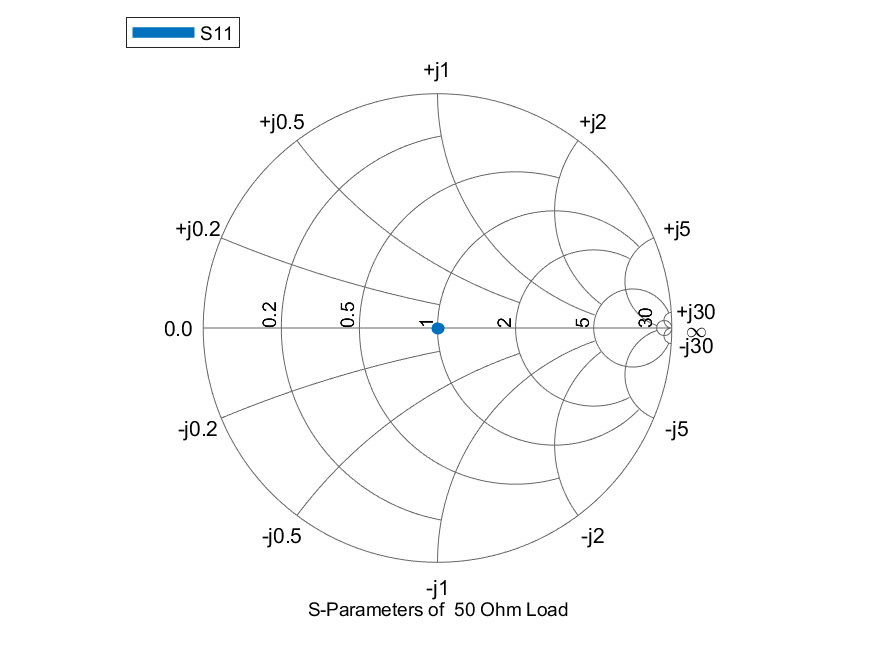
\includegraphics[width=0.3\textwidth]{load_smith_chart.png}
    \caption{\label{fig:load_smith} Smith Chart showing S\({}_{1,1}\) of 50 \(\Omega\) Load}
\end{figure}

\begin{figure}[hbp]
    \centering
    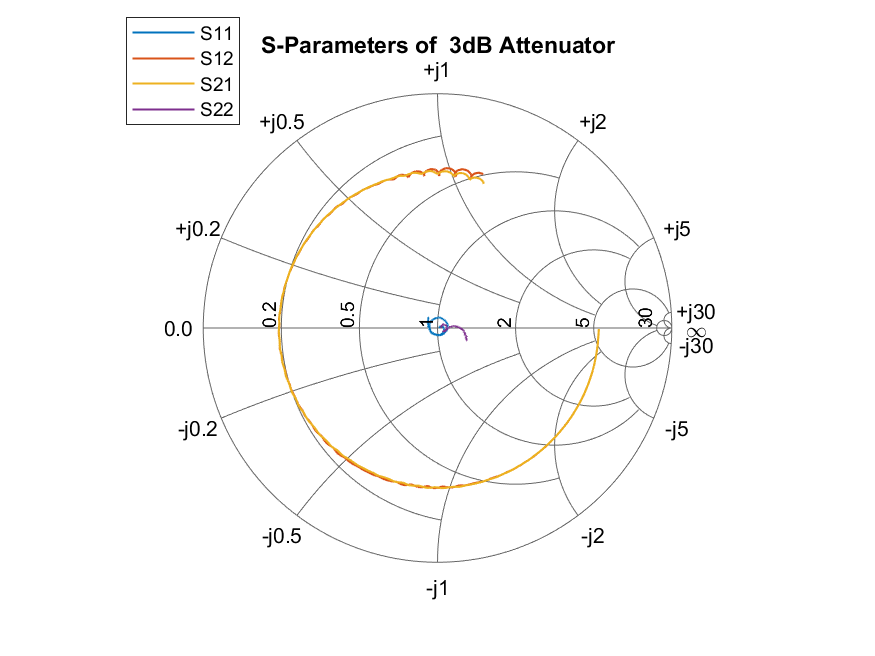
\includegraphics[width=0.3\textwidth]{3db_smith_chart.png}
    \caption{\label{fig:3db_smith} Smith Chart showing S-parameters of 3 dB attenuator}
\end{figure}

\begin{figure}[hbp]
    \centering
    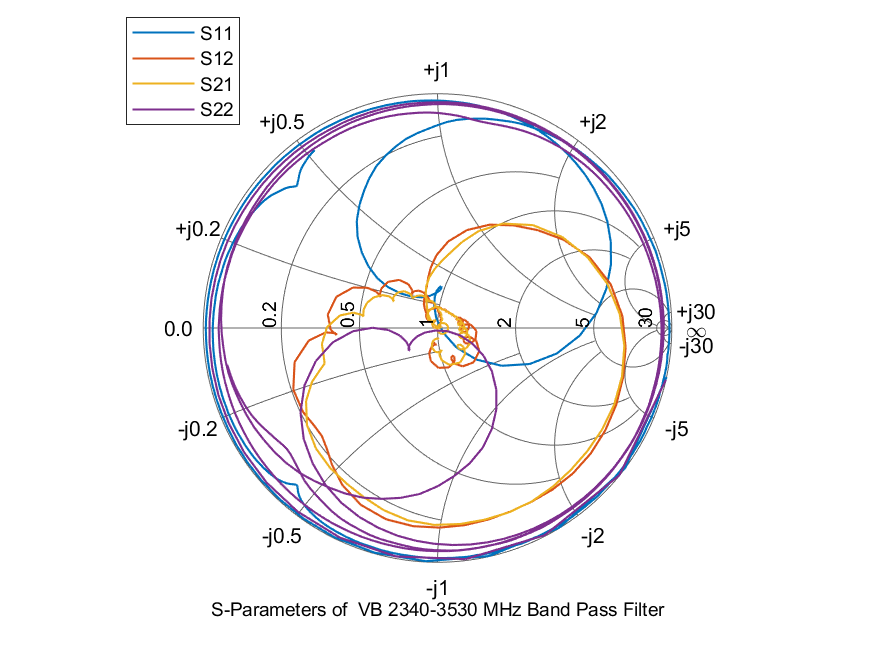
\includegraphics[width=0.3\textwidth]{band_pass_smith_chart.png}
    \caption{\label{fig:band_pass_smith} Smith Chart showing S-parameters of band pass filter}
\end{figure}

\begin{figure}[hbp]
    \centering
    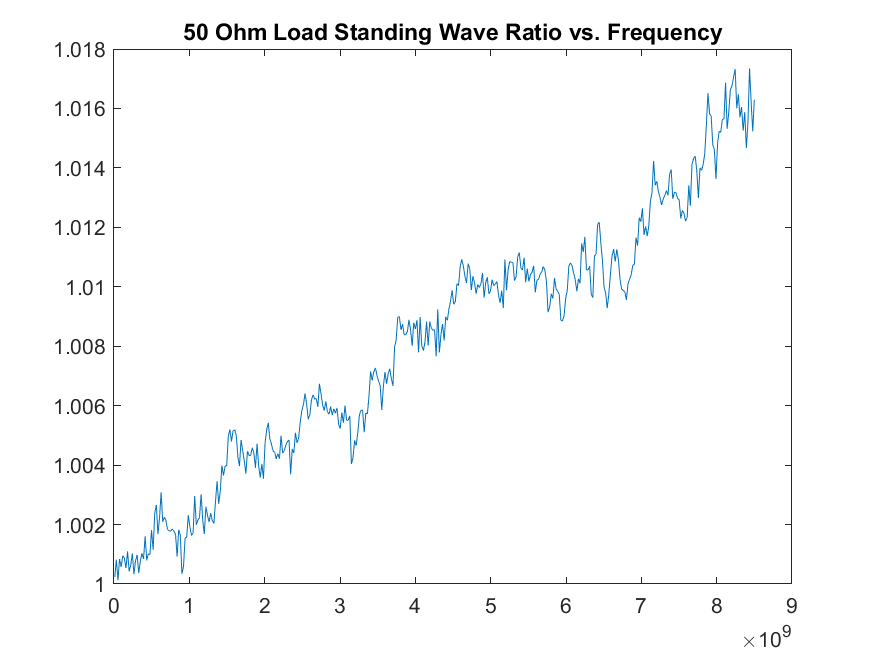
\includegraphics[width=0.3\textwidth]{load_swr.png}
    \caption{\label{fig:load_swr}  Standing Wave Ratio vs. Frequency  of 50 \(\Omega\) Load}
\end{figure}

\begin{figure}[hbp]
    \centering
    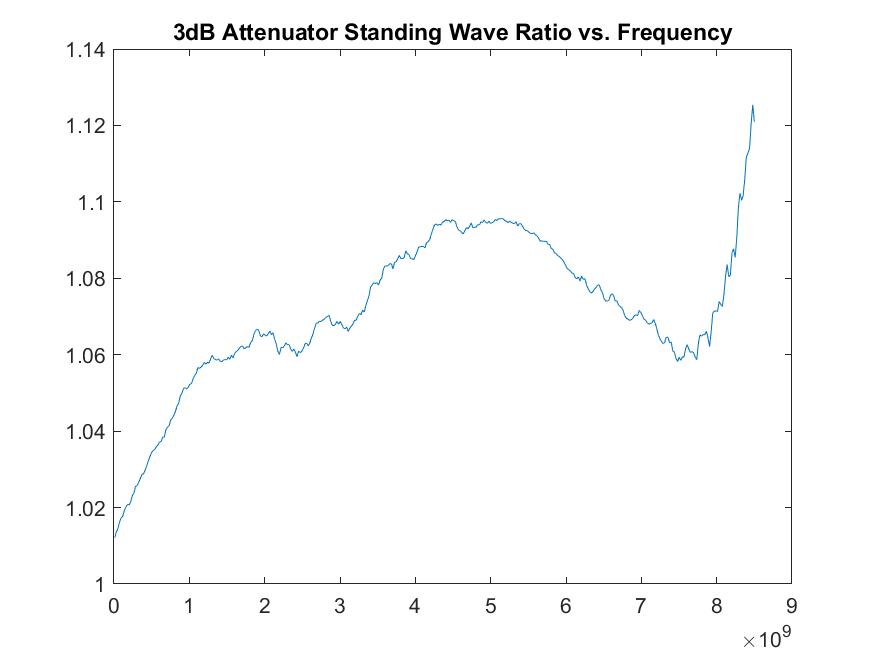
\includegraphics[width=0.3\textwidth]{3db_swr.png}
    \caption{\label{fig:3db_swr}  Standing Wave Ratio vs. Frequency  3dB Attenuator}
\end{figure}

\begin{figure}[hbp]
    \centering
    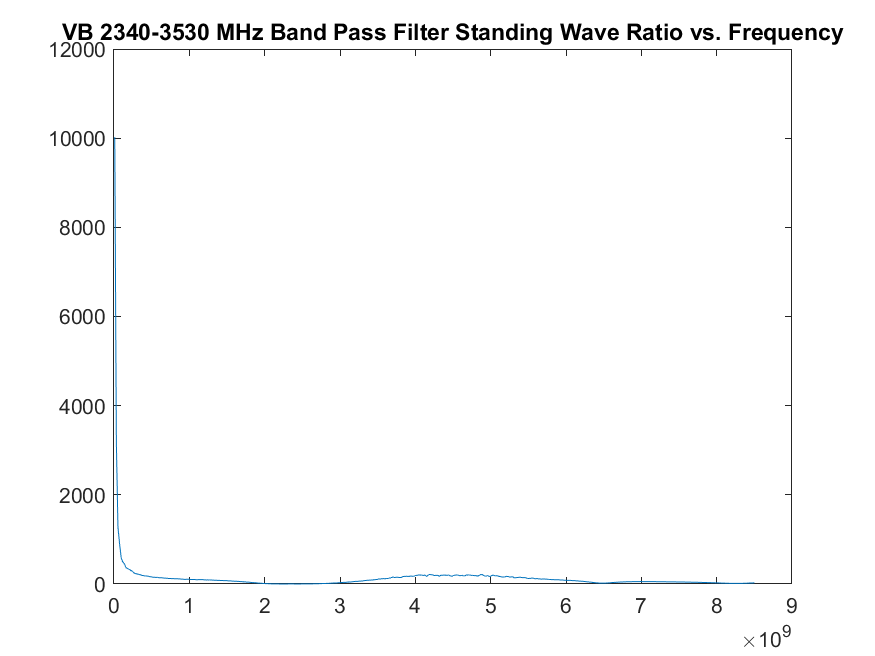
\includegraphics[width=0.3\textwidth]{band_pass_swr.png}
    \caption{\label{fig:band_pass_swr}  Standing Wave Ratio vs. Frequency  of Band Pass Filter}
\end{figure}

\begin{figure}[hbp]
    \centering
    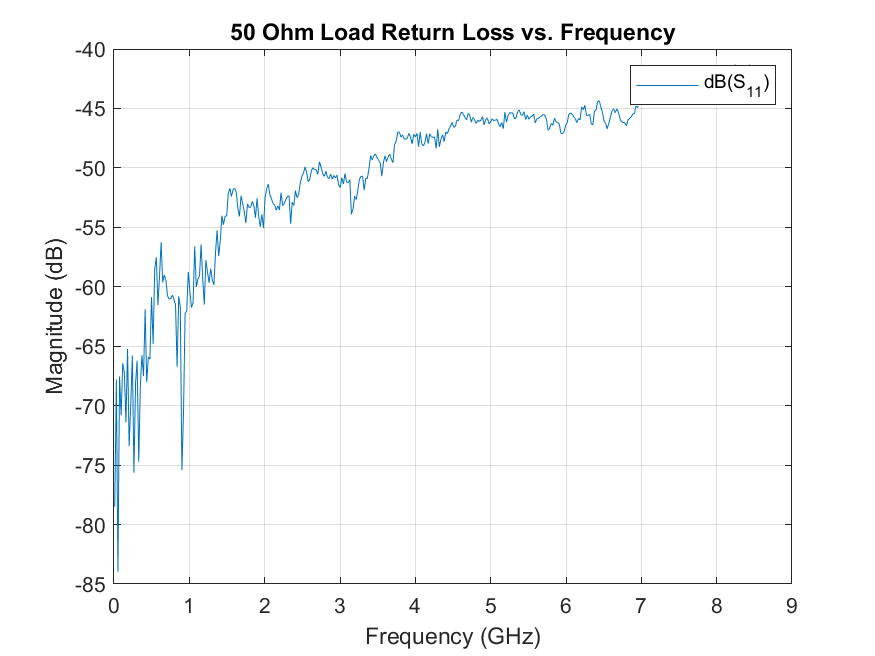
\includegraphics[width=0.3\textwidth]{load_rl.png}
    \caption{\label{fig:load_rl}  Return Loss vs. Frequency  of 50 \(\Omega\) Load}
\end{figure}

\begin{figure}[hbp]
    \centering
    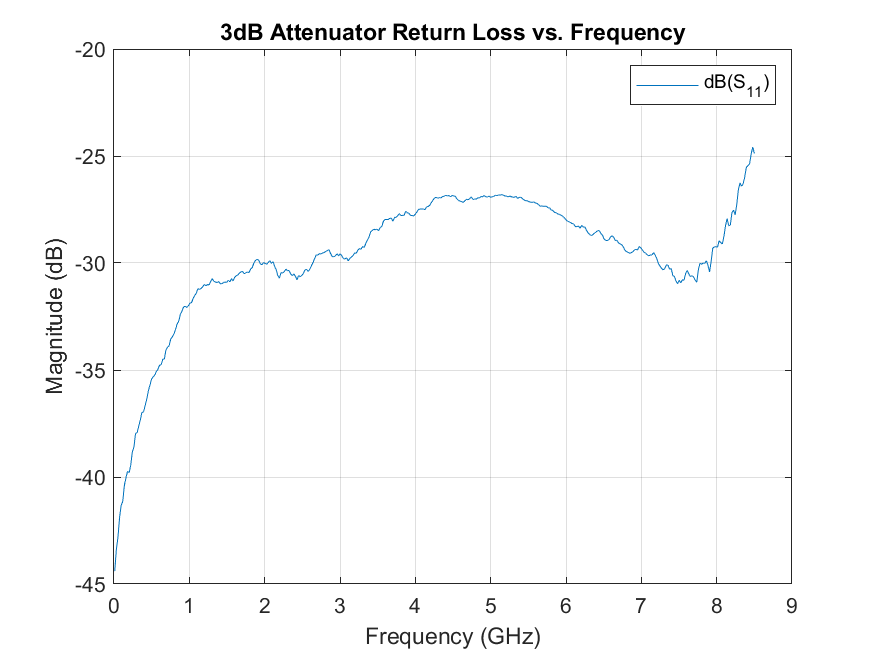
\includegraphics[width=0.3\textwidth]{3db_rl.png}
    \caption{\label{fig:3db_rl}  Return Loss vs. Frequency  of 3dB Attenuator}
\end{figure}

\begin{figure}[hbp]
    \centering
    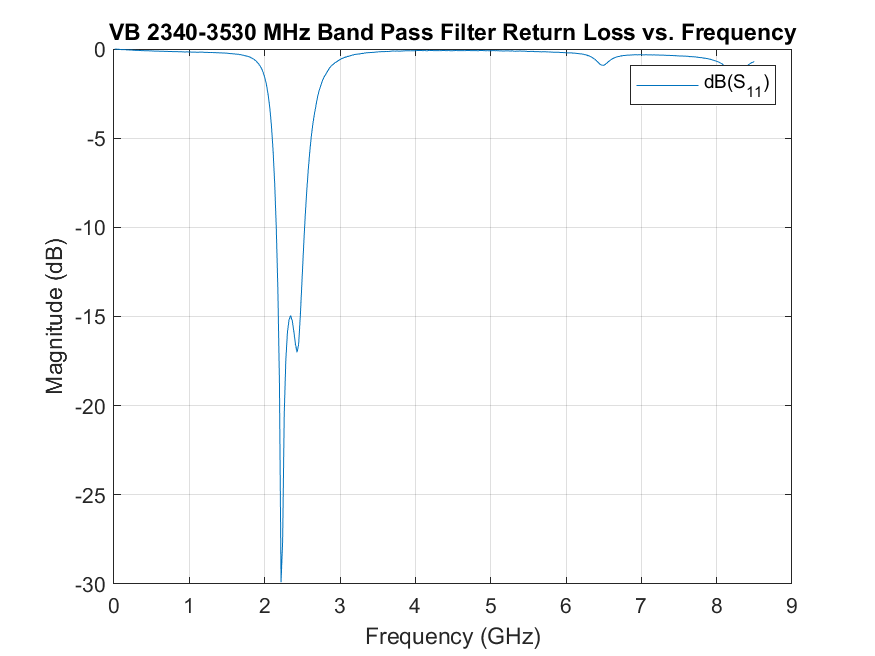
\includegraphics[width=0.3\textwidth]{band_pass_rl.png}
    \caption{\label{fig:band_pass_rl}  Return Loss vs. Frequency  of Band Pass Filter}
\end{figure}


\section{Discussion and Summary}

From this lab procedure, the effect of calibration as it relates to vector
impedance measurements has been extremely relevant. In order to accurately
measure devices across single or dual ports, SOLT calibration can be performed
in order to remove systematic error and account for the movement of the reference plane.

\subsection{Questions to Consider}

\textbf{Why do we need to perform vector impedance measurements to design microwave amplifiers?}

S-parameters/vector impedance measurements allow linear systems that operate at
high frequencies to be characterized by few parameters that can predict the
system's response. These fundamental parameters give the ability to predict how
multiple components will interact without actually testing how they interact
which facilitates design iteration time. These parameters  can predict gain,
loss, and the reflection coefficient of a group of components in a system.
Vector impedance measurements are fundamental to designing microwave amplifiers
because of their ability to describe a system at high frequency operating
conditions.

\textbf{What happens to our measurements if we do not achieve a “good” calibration?}

Because calibration such as SOLT mitigates systematic errors, not achieving a
``good'' calibration means that the systematic error maybe over or under
compensated for.  Poor calibration results in all measurements containing the
same systematic error.
\appendices
\section{Pre-Lab}
\textbf{Why do we use an SOLT calibration for a 2-port VNA calibration?}

Short Open Load Through (SOLT) calibration allows the VNA to properly account
for systematic error and thus its effects can be almost entirely removed.  It
is a common type of calibration that provides ``broadband'' calibration that is
easy to perform.

\textbf{How does a VNA work? (brief summary of how a VNA makes vector impedance measurements; Length: 1/2 page)}

A vector network analyzer (VNA) is comprised of a signal source, signal
separators, receivers, and processors. Most sources allow for a signal to be
swept across power or frequency. Signal separators allow different signal paths
to be analyzed and measured independently. The separators allow for the incident
signal to be measured and ``ratioed'' to the reflected and transmitted signals.
The signal are measured with a tuned receiver. This receiver mixes the signal
down to an intermediate frequency (IF) utilizing a local oscillator (LO). This
frequency usually  corresponds to the maximum frequency that the analog to
digital converter can handle accurately, at least twice the converters Nyquist
criterion.  The mixed down signal is passed through a bandpass filter to hone in
on the target signal. When the analog to digital convert processes the signal it
is likely passed on to a dedicated digital signal processor or other type of
computing chip. This chip further processes and formats the data to make it more
easily understood by humans. Several algorithms such as the Fast Fourier
Transform may be run to understand the frequency characteristics of the
signals. Notably, because the received signals correspond to 3 parts of the
flow: incident, reflected, and transmitted these digitized signals can be
measured and the ratio can be taken between them. This allows a variety of different
measurements to be conducted including S-parameters and Transmission/Reflection
Tests. Specifically S-parameters/Vector Impedance measurements can be
determined by performing mathematical operations between the incident, reflected
and transmitted signals in the processor.

% \section{Extra Photos}

\end{document}